\chapter{User Interface, Heads-Up Display, and Context Interaction}
\label{chap:hud}

\section{In-Window HUD Architecture}
Early graphics prototypes frequently clutter the developer console with stdout logs, disrupting visual immersion. To provide professional, in-engine telemetry with negligible rendering overhead, \textit{Matsuri Nights} features an \textbf{In-Window Minimal Heads-Up Display (HUD)} implemented in \texttt{src/ui/Hud.cpp}.

\subsection{Embedded \texorpdfstring{$256\times 256$}{256x256} Consolas Font Atlas}
To avoid complex external TrueType font parsing libraries (such as FreeType), the engine embeds an auto-generated $256 \times 256$ monochrome Consolas Bold font atlas as a static C++ array (\texttt{src/ui/FontAtlasData.h}):
\begin{itemize}
    \item \textbf{Dimensions:} 256 width, 256 height (65,536 bytes).
    \item \textbf{Glyph Grid:} 16 columns $\times$ 6 rows covering printable ASCII characters ($32 \dots 127$).
    \item \textbf{Cell Dimensions:} Cell width 16 pixels, cell height 24 pixels.
    \item \textbf{OpenGL Texture:} Uploaded once as a single-channel \texttt{GL\_RED} luminance texture.
\end{itemize}

\subsection{Batched 2D Orthographic Render Pass}
The HUD pass renders directly into the default framebuffer immediately prior to buffer swapping:
\begin{enumerate}
    \item Depth testing is temporarily disabled (\texttt{glDisable(GL\_DEPTH\_TEST)}), and alpha blending is enabled (\texttt{glBlendFunc(GL\_SRC\_ALPHA, GL\_ONE\_MINUS\_SRC\_ALPHA)}).
    \item The 2D vertex shader (\texttt{shaders/hud.vert}) applies an orthographic matrix mapping pixel coordinates $(x, y) \in [0, W] \times [0, H]$ onto NDC $[-1, 1] \times [1, -1]$:
    \begin{equation}
    x_{\text{ndc}} = \frac{2x}{W} - 1.0, \quad y_{\text{ndc}} = 1.0 - \frac{2y}{H}
    \end{equation}
    \item \textbf{Batched VBO:} Both translucent dark background panels and textured glyph quads are packed into a single interleaved vertex buffer:
    \begin{lstlisting}[language=C++, basicstyle=\ttfamily\scriptsize]
    struct HudVertex {
        float x, y;       // Screen pixel position
        float u, v;       // Atlas UV (or -1.0 for solid colored panels)
        float r, g, b, a; // RGBA color tint & opacity
    };
    \end{lstlisting}
    A single \texttt{glDrawArrays} call dispatches the entire UI overlay in less than $0.05\,\text{ms}$.
\end{enumerate}

\begin{figure}[htbp]
\centering
\IfFileExists{figures/ss_18_hud_overlay.png}{%
  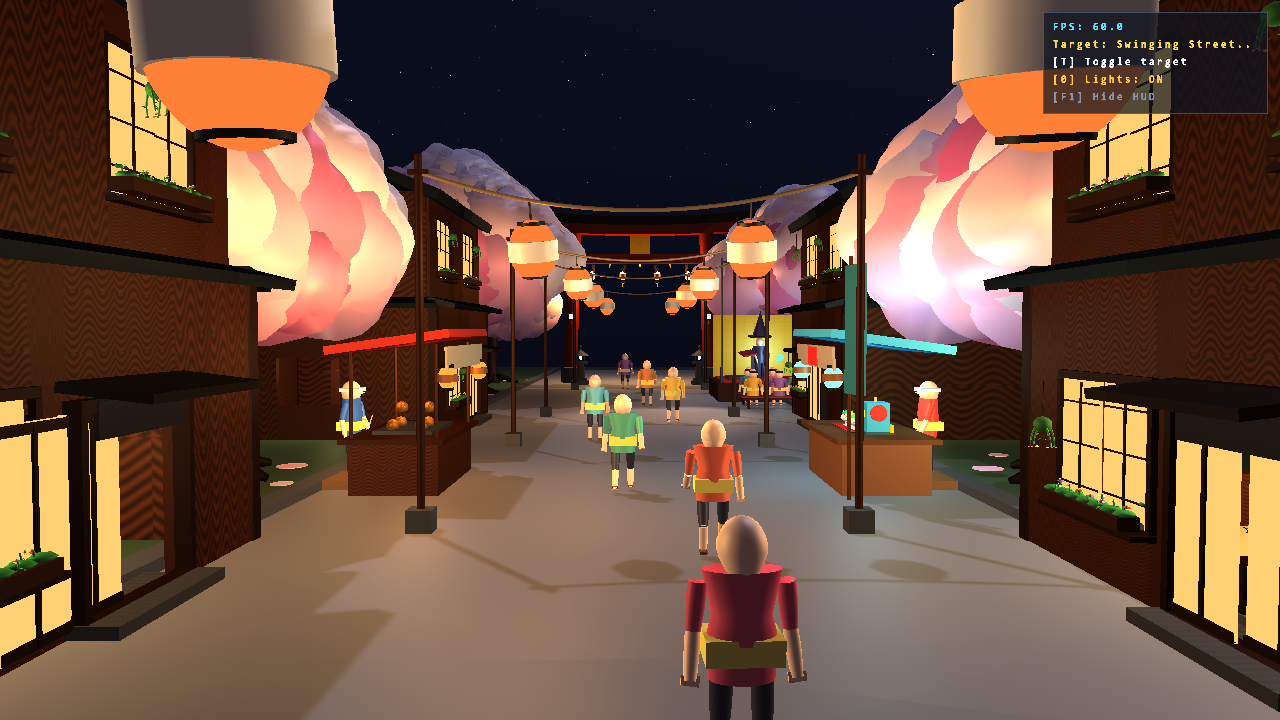
\includegraphics[width=0.68\textwidth]{figures/ss_18_hud_overlay.png}%
}{\fbox{ss\_18}}
\caption{In-window minimal HUD overlay displaying real-time FPS telemetry, active scene states, selected target metadata, and contextual control hints.}
\label{fig:hud_overlay}
\end{figure}

\section{Context-Sensitive Interaction System}
The interaction manager (\texttt{src/ui/InteractionManager.cpp}) tracks player position and spatial orientation relative to scene entities:
\begin{itemize}
    \item \textbf{Proximity Auto-Selection:} When the player walks within interaction range of any building, stall, or landmark, the entity is automatically highlighted on the HUD.
    \item \textbf{Contextual Action Hints:} When standing near a townhouse, the HUD dynamically displays:
    \begin{center}
    \texttt{[H] Slide Open/Close Shoji Door \quad\quad [G] Slide Open/Close Windows}
    \end{center}
    When approaching the stage, it displays \texttt{[M] Replay Magic Show Trick}.
    \item \textbf{Manual Selection Lock (Key T):} Pressing \textbf{T} locks selection onto a specific target, enabling live transformation manipulation. Pressing \textbf{Shift + T} unlocks selection back to proximity auto-mode.
\end{itemize}

\section{Live In-Engine Object Transformation Controls}
When an object is selected (via Key \textbf{T} or proximity), the user can translate, rotate, and scale it directly in the running viewport:
\begin{itemize}
    \item \textbf{3D Translation:} Keys \textbf{I / K} modify Elevation ($\pm Y$), \textbf{J / L} modify Lateral Axis ($\pm X$), and \textbf{U / O} modify Depth ($\pm Z$).
    \item \textbf{3D Rotation:} \textbf{Arrow Keys Up / Down} rotate Pitch ($\pm X$); \textbf{Arrow Keys Left / Right} rotate Yaw ($\pm Y$).
    \item \textbf{3D Scale:} Keys \textbf{+ / -} (or \textbf{[ / ]}) scale the object by $\pm 10\%$.
\end{itemize}
All modifications update local transform matrices immediately and propagate across child nodes, demonstrating real-time scene graph reactivity.
